\section{Redescription mining}
\subsection{Definition}
Redescription mining is a process of discovering a set of criteria that describe a subset of data in multiple, complementary ways.
In other words, it is a method of coming up with various ways to describe the same data or set of data.
It can be used to find novel links or patterns in huge collections of data in a variety of domains.

\begin{figure}[bt]
    \centering
    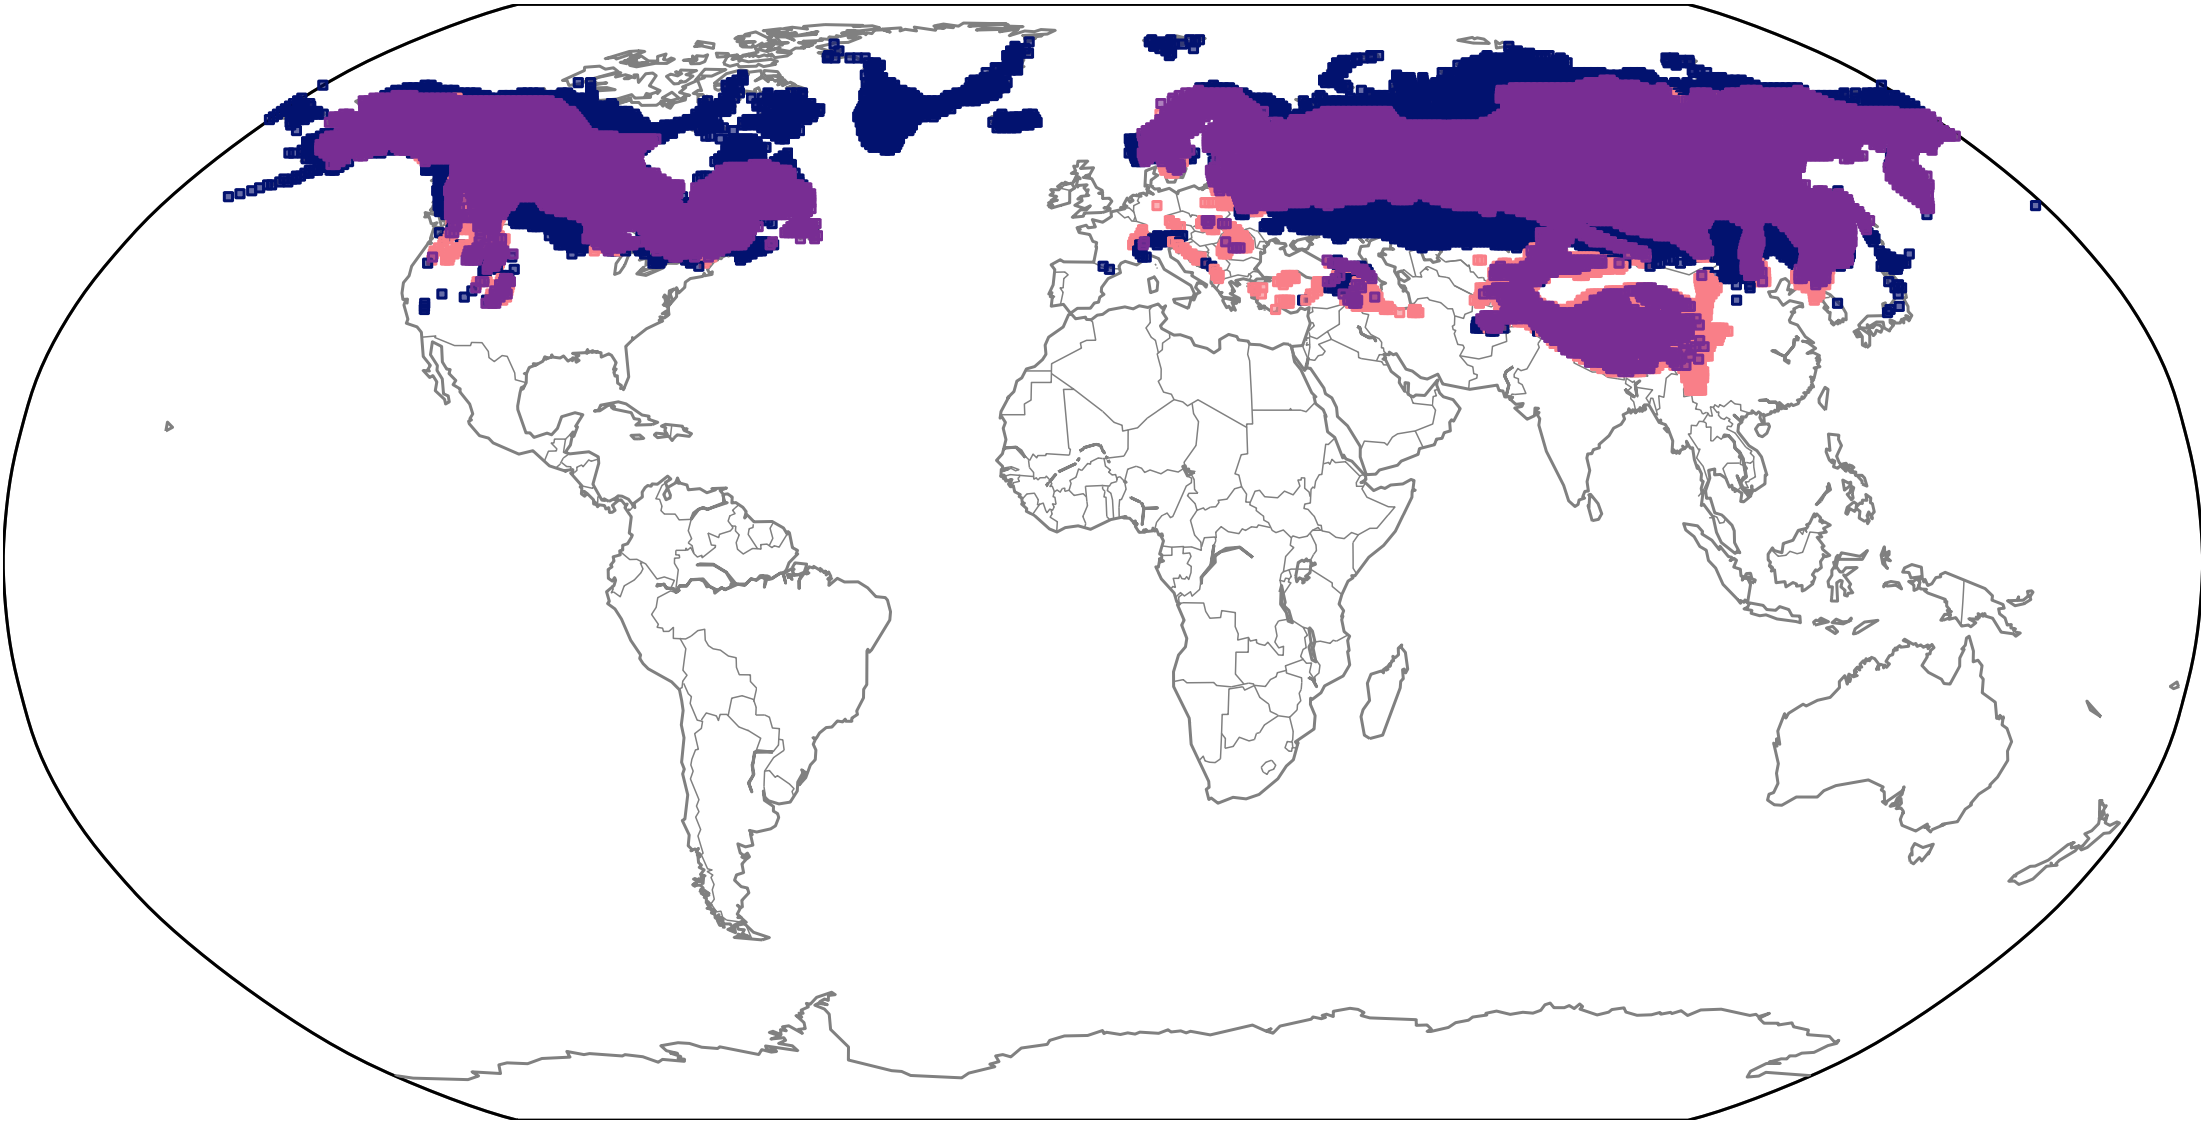
\includegraphics[width=10cm]{niche-finding}
    \caption{An example redescription plotted on a map, showing the areas inhabited by lynxes (light red and medium purple) and the areas where the maximum March temperature is between \SI{-24.4}{\degreeCelsius{}} and \SI{3.4}{\degreeCelsius{}} (dark blue and medium purple) \cite{galbrun2018redescription}}
    \label{fig:niche}
\end{figure}
A classic example of redescription mining application is in finding bio-climatic niches, or, in other words, relate the habitat of particular species or groups of species, to the local climatic conditions.
In this example, we want to describe geographic regions in terms of the fauna that inhabits them, on one hand, and in terms of the values of some climatic variables, on the other hand. In particular, the aim of redescription mining is to extract such pairs of descriptions automatically from a given dataset.
As a specific example, the method might return a redescription that states that areas where the maximum temperature in March is between \SI{-24.4}{\degreeCelsius{}} and \SI{4.3}{\degreeCelsius{}} are roughly the same as area inhabited by lynxes (see Figure~\ref{fig:niche}).
In this application, the aim is to help ecologists understand the impact of climate on the distribution of species.

\begin{table}[tb]
    \resizebox{\textwidth}{!}{%
    \begin{tabular}{|l|l|l|l|l|l|l|l|l|l|l|l|}
    \cline{1-6} \cline{8-12}
    \multicolumn{6}{|c|}{Species occurrences} &  & \multicolumn{5}{c|}{Climate}                                  \\ \cline{1-6} \cline{8-12} 
    Location ID   & mountain hare & \dots & Canada lynx   & Eurasian lynx  & \dots  &  & Location ID & \dots & max.\ March T.\ & avg.\ May P.\ & \dots \\ \cline{1-6} \cline{8-12} 
    \dots  & \dots & \dots & \dots   & \dots  & \dots &  & \dots  & \dots & \dots & \dots & \dots \\ \cline{1-6} \cline{8-12} 
    4652 & True  & \dots & True  & False & \dots &  & 4652 & \dots & 2   & 10  & \dots \\ \cline{1-6} \cline{8-12} 
    4653 & True  & \dots & False & True & \dots &  & 4653 & \dots & 3   & 40  & \dots \\ \cline{1-6} \cline{8-12} 
    \dots. & \dots & \dots & \dots   & \dots  & \dots &  & \dots. & \dots & \dots & \dots & \dots \\ \cline{1-6} \cline{8-12} 
    \end{tabular}%
    }
    \caption{An example dataset, represented as a pair of data tables with mapped rows. The left-hand side table records occurrences of various species, while the right-hand side table records the values of various bio-climatic variables such as temperature (T, in \si{\degreeCelsius{}}) and precipitation (P, in \si{\milli\meter}).}
    \label{tab:mammals-and-climate}
\end{table}


Here we follow the formalism of \cite{Galbrun-Methods}.
The redescription mining data model $\mathcal{D}$ is a tuple of 3 sets: $\left( entity\;\mathcal{E}, attributes\;\mathcal{A}, views\;\mathcal{V} \right)$.
Each entity $e \in \mathcal{E}$ is associated with a set of attributes $a \in \mathcal{A}$.
The attributes are partitioned into disjoint \emph{views} $v \in \mathcal{V}$ that correspond to logical groups of attributes. Each view can be thought of as a data table, where the columns represent the attributes, and the rows represent the entities, which map across the different tables.
Usually, the data contains 2 datasets, one left-hand side and one right-hand side data.
In the bioclimatic-niche finding example above, the entities are geographic locations and the views correspond to species occurrences and climate, respectively.
That is, one view contains attributes that each record the presence or absence of a specific species in each location, whereas the other view contains attributes that each record the value taken by a specific climatic variable in each location.
This can be represented as a pair of tables, as shown in Table~\ref{tab:mammals-and-climate}.

Then, a description, or query, is a logical formula over attributes.
The query can be evaluated for each entity, and returns a Boolean value that indicates whether the entity satisfies the query conditions.
The support of a query is the set of entities that satisfy the query.
A redescription is then a pair of queries, respectively over attributes from distinct views, having sufficiently similar supports \cite{galbrun2018redescription}.
In the bioclimatic-niche finding example above, a redescription consists of a query over species occurrences and a query over climatic variables, respectively, that are satisfied in roughly the same locations.

For a redescription to satisfy the conditions, it must have similar supports between the two queries.
The similarity of the two queries $p$ and $q$ is denoted as $\sim$.
We can use the Jaccard distance to determine the similarity between the supports of the two description.
The Jaccard distance is based on the \acl{JSI}.

\begin{definition}[\acl{JSI} \citep{galbrun2018redescription}]
    The Jaccard (similarity) index J between the supports of two descriptions p and q is defined as below:

    \begin{equation}
        J(p, q) = J(supp(p), supp(q)) = \cfrac{\left|supp(p)\cap supp(q)\right|}{\left|supp(p)\cup supp(q)\right|}
    \end{equation}
\end{definition}

The requirement to calculate $J$ is obviously that none of $supp(q)$ and $supp(p)$ equals $\emptyset$.

\begin{definition}[Jaccard distance \citep{galbrun2018redescription}]
    The Jaccard distance is then defined as:

    \begin{equation}
        1 - J(p, q) = 1 - \cfrac{\left|supp(p)\cap supp(q)\right|}{\left|supp(p)\cup supp(q)\right|}
    \end{equation}
\end{definition}

Clearly, the smaller the distance is, the more accurate the redescription is.
When the distance between the two queries equals to $0$, the redescription is called \textit{exact}, and is denoted as $p \equiv q$.

From here, we can formulate the formal definition of the redescription.

\begin{definition}[Redescription \citep{galbrun2018redescription}]
    A redescription in query language $\mathcal{Q}$ over data $\mathcal{D}$ with similarity $\sim$ is a pair of query $(p, q) \in \mathcal{Q} \times \mathcal{Q}$ such that

    \begin{equation}
        p \sim q \text{ and } views(p) \cap views(q) = \emptyset
    \end{equation}
\end{definition}

\subsection{Redescription mining algorithms}
Different redescription mining algorithms have been proposed, that use different strategies, handle different types of attributes and allow different types of constraints on the queries \cite{galbrun2018redescription}.
There are two main categories of redescription mining algorithms: exhaustive and heuristic.
In the scope of the current thesis, we will be focusing on the exhaustive algorithms.

The most popular strategy of exhaustive redescription mining algorithms is \ac{MAP}.
The idea is quite simple, first we mine for all possible queries, then we will try to pair them together and see if their supports have big enough overlaps.
If the overlap between the two queries is bigger than a certain threshold, we then have found a redescription.

The \ac{MID} algorithm is an algorithm that follow the \ac{MAP} strategy.
We can have a look at the pseudocode of the \acl{MID} in Algorithm \ref{alg:MID}.
The mining for queries steps is in line 2, where the paring part is at line 12.

Recall that in statistic, p-value is the probabilities of the null hypothesis to be true.
The null hypothesis in this case is that the supports of a query is small.
The reason this is the hypothesis is that the chance of two disjoint small support sets to have overlap are small.

\begin{algorithm}[tb]
    \caption{Sketch of the \algMID{} algorithm \citep{galbrun2018redescription}.}
      \label{alg:MID}
    \begin{algorithmic}[1]
    \small
      \Require Two Boolean data tables $\Table_1$ and $\Table_2$, similarity $\similar$, maximum \pvalue{} $p_{\max}$, number of queries to select $N$, and maximum level $\kappa$.
      \Ensure Redescriptions $\mathcal{R}$.
      \For{side $i \in \{1, 2\}$} %\Comment{for each view separately}
       \State $\Queries^{(0)}_i \gets \{ \query : \query$ is a closed frequent itemset from $\Table_i$ or its negation and $ \pvalue(\query) \leq p_{\max}\}$ \label{alg:MID:mine} %\Comment{computing the \pvalue{} for the independent items \textit{null-model}}
       \State $\Queries^{(1)}_i \gets$  $N$ queries with the lowest \pvalue from $\Queries^{(0)}_i$ 
       \For{level $k \in \{1,\dots,(\kappa-1)\}$}
         \State $\Queries^{(k+1)}_i \gets \Queries^{(k)}_i$
         \For{operator $\lop \in \{\land, \lor\}$} % \Comment{combine queries using conjunctions and disjunctions}
            \State $\Queries^{(k+1)}_i \gets \Queries^{(k+1)}_i \cup \{ \query \lop \query' : \query, \query' \in \Queries^{(k)}_i, \pvalue(\query \lop \query') \leq p_{\max}\}$ \label{alg:MID:combine}
      \EndFor
       \State $\Queries^{(k+1)}_i \gets$  $N$ queries with the lowest \pvalue from $\Queries^{(k+1)}_i$ \label{alg:MID:filter}
      \EndFor
      \EndFor
      \State $\mathcal{R} \gets \{(\lquery, \rquery) \in \Queries^{(\kappa)}_1 \times \Queries^{(\kappa)}_2  : \lquery \similar \rquery\}$ \label{alg:MID:pair} %\Comment{collect query pairs across the views with sufficient accuracy}
      \State \textbf{return} $\mathcal{R}$
    \end{algorithmic}
\end{algorithm}

We can see that the \acl{arm} algorithms contribute an important part of the foundation of this redescription mining algorithm category.
Often times, a suitable \ac{fim} algorithms is the key to create a redescription mining algorithm for a specific problem.
For example the CHARM-L \citep{zakihsiao2005}, which is a \ac{fim} algorithm that can construct the closed itemset lattice.
The CHARM-L algorithm was then utilized to develop a redescription mining algorithm to find the exact conditional redescriptions for the lattice \Citep{zakimohammed2005}.
In the paper, three classes of redescription was formulated: exact, conditional, and approximate.
An exact redescription has a Jaccard distance = 0, while an approximate redescription has a Jaccard distance > 0.
A conditional redescription is derived from an approximate redescription and turned into an exact redescription by supplying additional constraints to the queries.
For instance, we have 2 queries $p$ and $q$ forming a redescription $(p \similar q)$ with a Jaccard distance distance > 0.
By introducing an additional constraint to both queries: $(p \cap r)$ and $(p \cap r)$, $(p \cap r) \similar (p \cap r)$ could have a Jaccard distance = 0.
This is denoted by $(p \similar q \mid r)$ where $p$, $q$, and $r$ are queries over some disjoint view $v \in \mathcal{V}$.
